\section{The solution}
\label{sec:middleware_architecture}

% Description of the overall architecture designs
% Argue for tactics used to archieve the QASes
% Discuss the trade-offs

This section describes the design of a prototype, which will be used to test if the selected architecture supports the quality attributes.

The initial candidates for the architecture, based on the research articles from chapter \ref{sec:related_work}, pointed towards implementing the system in a micro-service pattern or an event-driven pattern.
The conclusion was to use a micro-service pattern for overall communication between each system and within the micro-service pattern, to implement the production system with the event-driven software architecture. 
By using an event-driven architecture for the conveyor belt and its sensors, the system becomes capable of sharing real-time data, while adapting to changes if necessary. via asynchronous communication. 
By using a message bus for communication, the individual parts can remain loosely coupled increasing the overall interoperability of the system, while the different system components, become individually scalable. The downside to using these architectural patterns is the increased complexity in implementation. While the architecture behind the conveyor belt does not require a lot of different components, if the production later needs to add additional features, the complexity could become problematic.
\\
The entire system consists of many individual services, ranging from log collection to an inventory management system. Each system contains several sub-systems with different purposes see figure \ref{figure:2}.
\begin{figure}[ht]
    \centering
    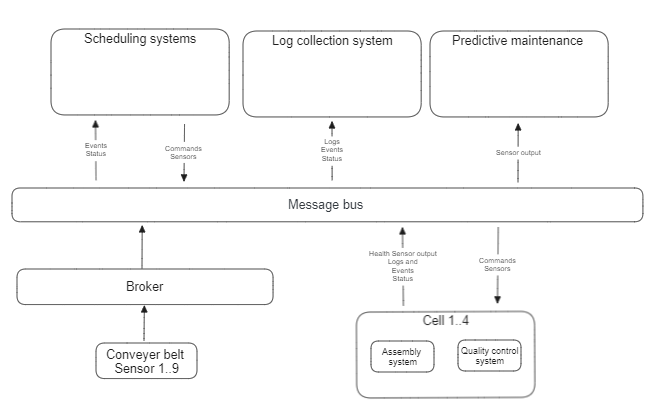
\includegraphics[scale=0.5]{Images/OverallArchitecture.png}
    \caption{The physical production layout}
    \label{figure:2}
\end{figure}


\
Designing the architecture as a whole and making design decisions for each system, would be too time-consuming and out of scope, considering the purpose is to create a testable prototype for an I4.0 production. 
As a result, the proposed solution will solely focus on the production system.

\subsection{Designing the production}
The physical production consists of 4 cells, each adding 1 additional part to the pen. Between these cells, there are sensors, which tell the next cell when the pen is ready. 
An illustration can be seen in figure \ref{figure:3}. Cells one and two operate in parallel while three and four operate sequentially as defined in \cite{torben21}.

\begin{figure}[ht]
    \centering
    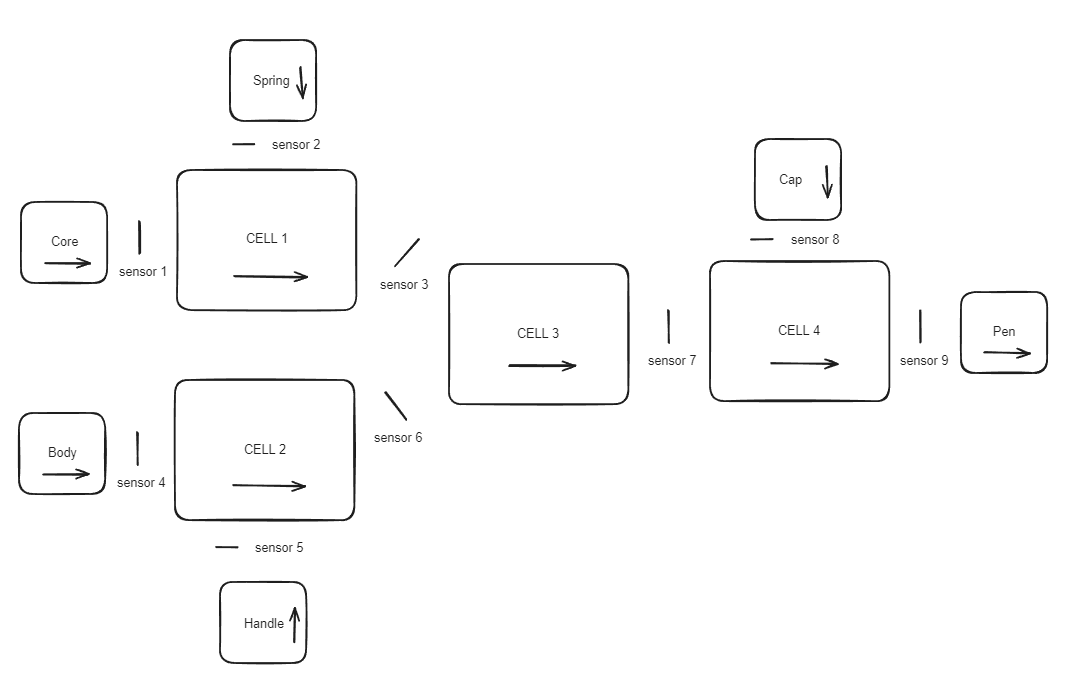
\includegraphics[scale=0.3]{Images/ProductionLayout.png}
    \caption{The physical production layout}
    \label{figure:3}
\end{figure}

Each cell contains a robotic system responsible for assembling or combining parts to create the pen. The cells contain several sensors ranging from when the pen is ready for further assembling to collecting health data, from the cell. By having sensors collecting health data frequently, it should become possible to predict maintenance and investigate why errors occur.
\
\subsubsection{Message Bus}
To manage this large quantity of data, the event-driven architecture becomes relevant. By implementing a message bus to manage the data flow within the system, each cell keeps its interoperability and stays individually scalable. \\ 
The message bus is responsible for receiving all the data from the different sensors and creating topics, where the relevant recipient can subscribe to receive the data.
For the production system, several MOMs (Message Oriented Middleware) were considered. According to \cite{Message-orientedMiddleware} the 4 most prominent within production systems are: 
MQTT, AMQP, and Kafka, which are all based on a broker, and ZeroMQ, which is brokerless. \\
Kafka has an edge over the others, due to the ability to replay messages:
“A unique approach having durable saved message streams and the ability to jump back and forth is taken by Kafka”\cite{Message-orientedMiddleware}. 
Kafka does this better than the other communication patterns while also allowing multiple publishers to write on the same topic.

Kafka is well-suited for real-time data streaming and event-driven architectures, while MQTT is tailored for lightweight, efficient communication in IoT scenarios. For that reason, each sensor between the cells will use the MQTT message bus to keep it lightweight and limit hardware usage. Kafka will mainly be responsible for handling the enterprise part of the system. 
However, a bridge/proxy between MQTT and Kafka will be created to analyze and save the data from the cells. 
Using both Kafka and MQTT collaboratively within the systems, allows the architecture to reap the benefits of both keeping the sensors lightweight, and having the Kafka capabilities for the rest of the system.
Working collaboratively with Kafka and MQTT has been implemented successfully before as seen in \cite{HiveMQTTvsKafka}.
While the sensors between cells will be communicating using the MQTT bridge, each individual cell will be transmitting its data directly to Kafka. 
\\
\subsubsection{Database Choice}
The production management system itself, will not have its own database, but the log data from the sensors still needs to be stored. This responsibility lies within the log collection system, which collects the data from Kafka via. an internal API. The data is then stored within a time series\cite{timeseries_db} database for later or ongoing analysis.
By storing this data the system becomes able to analyze itself in various ways. By continually checking the data sent from the sensors, it becomes possible to create a predictive model, which makes fault prevention possible. In the case a fault occurs, it should be detected quickly by monitoring the heartbeat continuously, through the data sent.

